\title{Warm-Up, September 26th, 2024 (INTD262)}
\author{Dr. Jordan Hanson - Whittier College Dept. of Physics and Astronomy}
\date{\today}
\documentclass[12pt]{article}
\usepackage[margin=1.25cm]{geometry}
\usepackage{hyperref}
\usepackage{graphicx}
\usepackage{amsmath}
\usepackage{subcaption}
\begin{document}
\maketitle

\small

\section{Chapter 3 of \textit{Science in Latin America}}

\begin{figure}[ht]
\centering
\begin{subfigure}{0.125\textwidth}
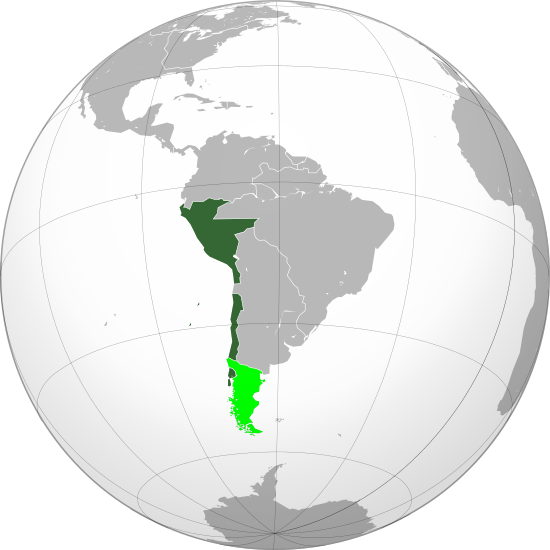
\includegraphics[width=\textwidth]{vice_peru.png}
\caption{\label{fig:1a}}
\end{subfigure}
\begin{subfigure}{0.125\textwidth}
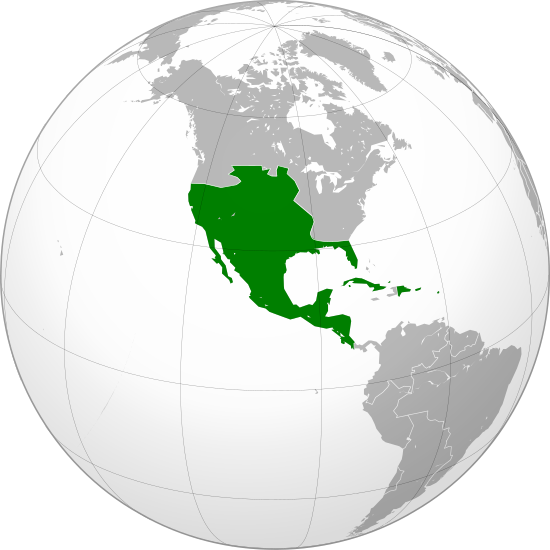
\includegraphics[width=\textwidth]{vice_nuevaespana.png}
\caption{\label{fig:1b}}
\end{subfigure}
\begin{subfigure}{0.125\textwidth}
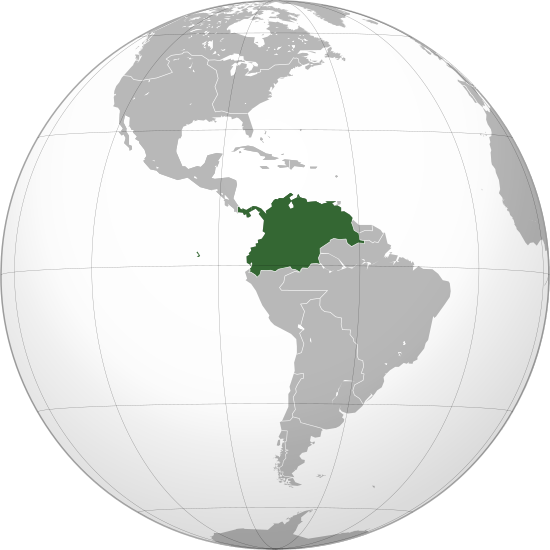
\includegraphics[width=\textwidth]{vice_nuevagranada.png}
\caption{\label{fig:1c}}
\end{subfigure}
\begin{subfigure}{0.125\textwidth}
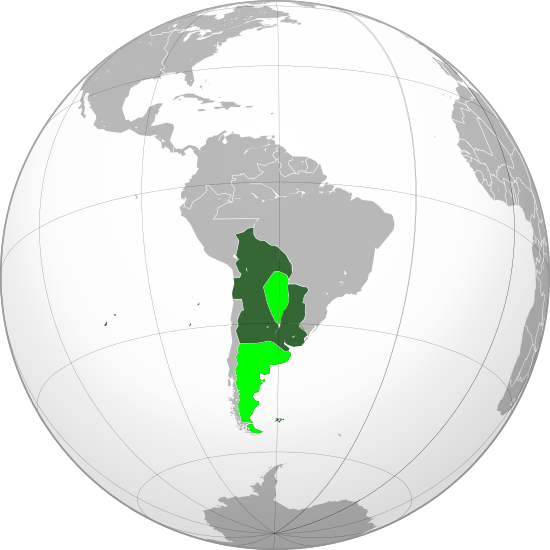
\includegraphics[width=\textwidth]{vice_riodelaplata.png}
\caption{\label{fig:1d}}
\end{subfigure}
\caption{\label{fig:1} Maps depicting \textit{virreinatos} in Latin America, 17th and 18th centuries.}
\end{figure}

\begin{enumerate}
\item (a) In what viceroyalty (Fig. \ref{fig:1}) was the city of Santa Fe de Bogot\'{a}? (b) Discuss the scientific implications of the ``half century-long polemic on Copernican theories, which started in 1773 between Jos\'{e} Celestino Mutis and the Dominican Congregation of Santa Fe de Bogot\'{a}. (c) In 1783, the Expedici\'{o}n Bot\'{a}nica began in Santa Fe.  What were some of its goals and achievements? \\ \vspace{2cm}
\item (a) In what viceroyalty (Fig. \ref{fig:1}) was the city of Quito? (b) List several goals of the expedition of Charles de la Condamine, Antonio Ulloa, and Jorge Juan to Quito and the surrounding regions. \\ \vspace{2cm}
\item (a) In what viceroyalty (Fig. \ref{fig:1}) was the city of Caracas? (b) In 1767, the Jesuit order was expelled from the Spanish colonies.  The Dominican order recovered authority over some colleges and universities.  What was the implication for science? \\ \vspace{2cm}
\item List some of the scientific achievements of Jos\'{e} Celestino Mutis in Nueva Granada.
\end{enumerate}

\end{document}
